\chapter{Project schedule}
\label{chap:schedule}

In this section, we will include an updated project schedule from the one we provided for milestone 1. Upon submission of the milestone 1 document, we were offered feedback that stated that our original Gantt Chart contained sprints that were too long and contained a lack of notable slippage time. We have reflected the constructive criticism we received within our updated Gantt Chart. It now includes a higher number of, but smaller sprints. Each sprint contains plans to develop code that will progress the project, along with integration testing to ensure that each feature we add to the project is functional. Within each sprint, we also allowed for slippage time where possible in an attempt to minimise the effects of the arising of any risks detailed within our risk analysis section in section \ref{sec:risk}.

Whilst developing the software for the project up to this point, it has become more clear to us what work needs doing at each stage of the development of our product. This has been reflected in our Gantt Chart, where we are more specific with each software development task that needs completing, as well as being more stringent with the time period we have assigned to completing each task. On the topic of being more strict with the time assigned to the completion of each task in the Gantt Chart, it is imperative that we have done this due to the delays we faced in hardware procurement, and therefore the delays we faced in being able to develop software. 

In figure \ref{fig:gantt_chart}, we can see the tasks remaining on the left and their visualisations on the right, along with the highlighted critical path. We split the work left to be completed into 3 Sprints, as we are utilising the scrum methodology. The main differences between the old and updated Gantt Charts are that we changed Sprint 3 from the original Gantt Chart to a group of smaller and more specific sprints, as well as detailing more specific tasks to be completed as well as assigning more strict time periods to those tasks. 

The plans for each Sprint has changed slightly to reflect the delays we have experienced in being able to begin development of the product. We now aim to meet every Thursday to discuss progress made in the previous week, as well as what features need to be developed next. We have also included overlap of some tasks as we aim to split the workload between team members to allow for more efficient project progression.


\afterpage{%
    \clearpage% Flush earlier floats (otherwise order might not be correct)
    \thispagestyle{empty}% empty page style (?)
    \begin{landscape}% Landscape page
        \centering % Center table

        \section{Gantt Chart}

          \begin{figure}[ht!]
            \hspace{-7.5em}
            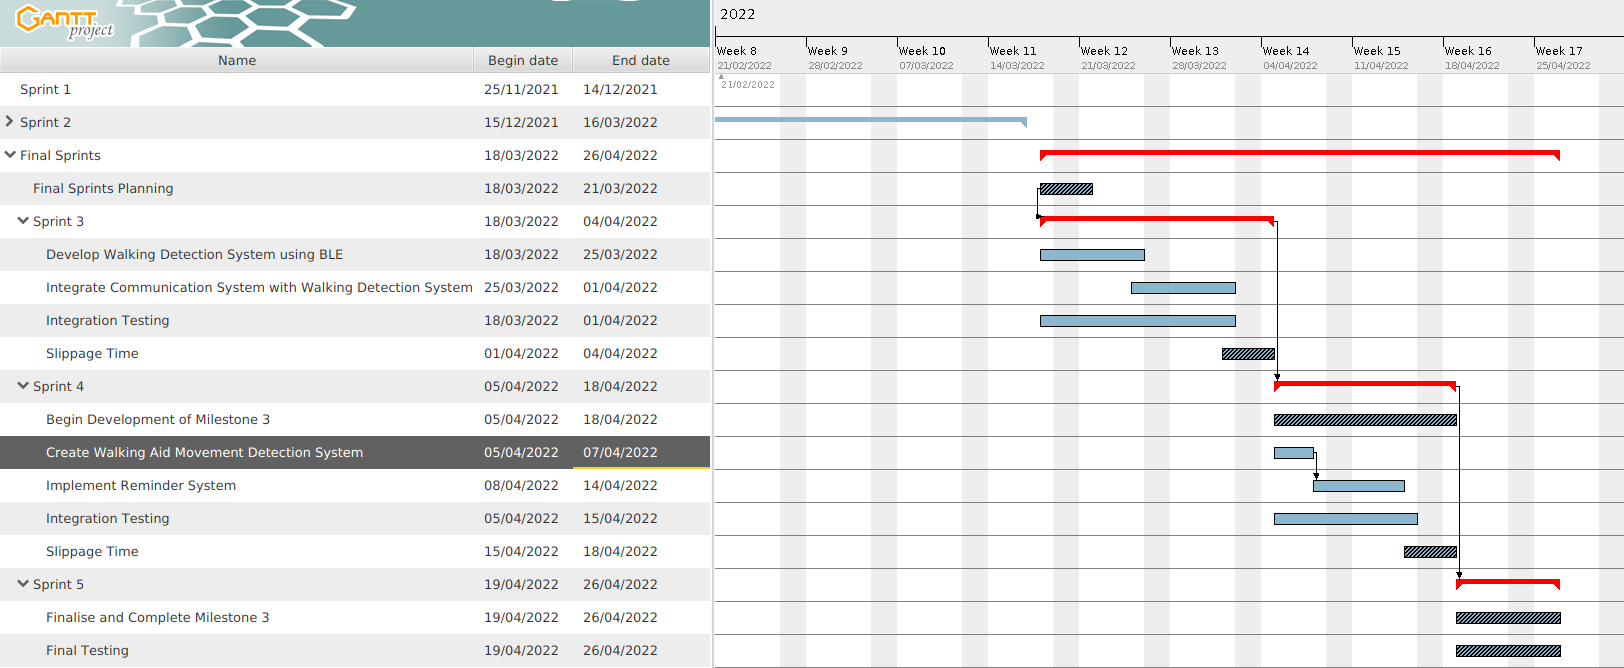
\includegraphics[width=2\textwidth]{./figures/m2.png}
            \caption{Our updated gantt chart}
            \label{fig:gantt_chart}
          \end{figure}

        \pagebreak

    \end{landscape}
    \clearpage% Flush page
}
